\begin{figure}
\begin{center}
\resizebox{\linewidth}{!}{
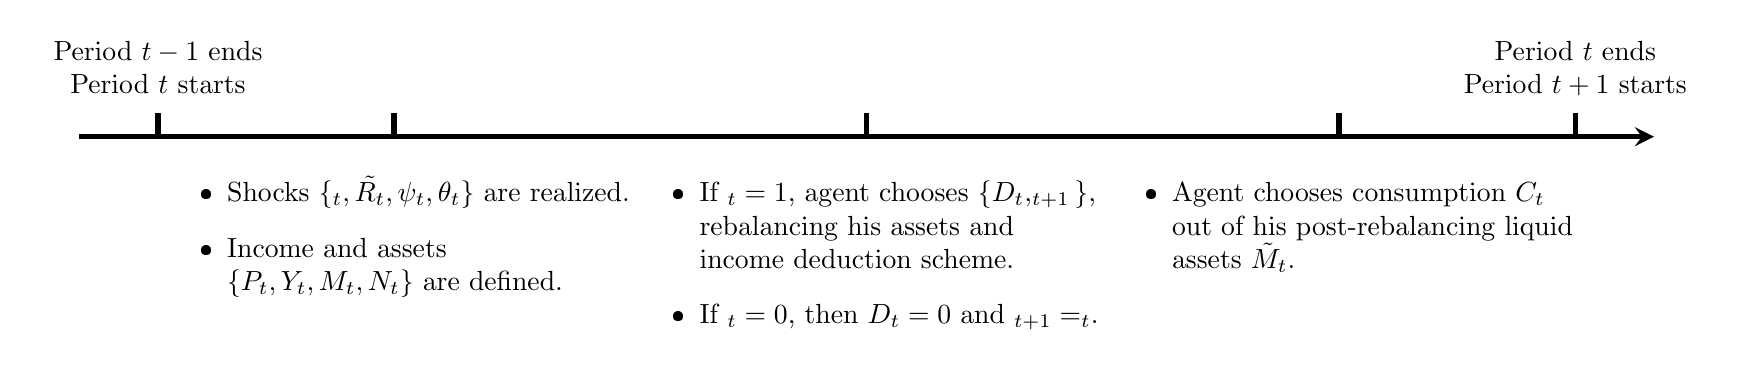
\begin{tikzpicture}
\usetikzlibrary{calc}

% draw arrow
\coordinate (start) at (-3,0);
\coordinate (end) at (17,0);

\draw [line width=2pt, -stealth] (start) -- (end);

% Priod ticks
\coordinate (period_s) at ($(start) + (1,0)$);
\coordinate (period_st) at ($(period_s) + (0,0.3)$);
\coordinate (period_e) at ($(end) - (1,0)$);
\coordinate (period_et) at ($(period_e) + (0,0.3)$);

\draw [line width=2pt] (period_s) -- (period_st);
\node [anchor=south] at (period_st.north) {\begin{tabular}{c}
Period $t-1$ ends \\ Period $t$ starts
\end{tabular}};

\draw [line width=2pt] (period_e) -- (period_et);
\node [anchor=south] at (period_et.north) {\begin{tabular}{c}
Period $t$ ends \\ Period $t+1$ starts
\end{tabular}};

% You can use `foreach` to improve the following codes
\coordinate (s0) at (1,0);
\coordinate (t0) at ($(s0)+(0,0.3)$);
\coordinate (s1) at (7,0);
\coordinate (t1) at ($(s1)+(0,0.3)$);
\coordinate (s2) at (13,0);
\coordinate (t2) at ($(s2)+(0,0.3)$);

% draw ticks
\draw [line width=2pt] (s0) -- (t0);
\node [anchor=south] at (t0.north) {};

\draw [line width=2pt] (t1) -- (s1);
\node [anchor=south] at (t1.north) {};

\draw [line width=2pt] (t2) -- (s2);
\node [anchor=south] at (t2.north) {};

% add texts
\node [anchor=north, align=left, text width=6cm] at (s0.south) {
\begin{itemize}
\item Shocks $\{\Adj_t,\tilde{R_t}, \psi_t, \theta_t\}$ are realized.
\item Income and assets $\{P_t, Y_t, M_t, N_t\}$ are defined.
\end{itemize}
};

\node [anchor=north, align=left, text width=6cm] at (s1.south) {
\begin{itemize}
\item If $\Adj_t=1$, agent chooses $\{D_t,\Contr_{t+1}\}$, rebalancing
his assets and income deduction scheme.
\item If $\Adj_t = 0$, then $D_t =0$ and $\Contr_{t+1} = \Contr_t$.
\end{itemize}
};

\node [anchor=north, align=left, text width=6cm] at (s2.south) {
\begin{itemize}
\item Agent chooses consumption $C_t$ out of his post-rebalancing
liquid assets $\tilde{M}_t$.
\end{itemize}
};
\end{tikzpicture}
}

\caption{Summary of the Model's Timing}\label{fig:Timing_diagram}
\end{center}
\end{figure}